\chapter{Cross Section Measurement}

The cross section measurement procedure and results are explained in this section.
After applying selection criteria and kinematic reconstruction, one can count the events to determine
the rate of $t\bar{t}$ production process.

The cross sections were measured double differentially in bins of the kinematic variables of the event.
A binning choice is explained in the first section.
The two dimensional unfolding was applied to correct for the detector effect and fluctuations, which is described
in the second section of this chapter.
The double differential cross sections and their definitions are shown in the last section of the chapter.
% \section{Selection of Binning}\label{sec:binning}

\section{Unfolding of the Experimental Results}\label{sec:unfold}

This study is performed as counting of events which fulfill certain criteria (e.g. given in chapter \ref{chapt:event_selection} and 
chapter \ref{chapt:kinReco}) and grouping them into bins (as described in sec. \ref{sec:binning}). However, a finite precision
of experimental apparatus and reconstruction algorithms may lead to incorrect measurement of kinematic properties of the event.
Thus, some fraction of events may be reconstructed in the wrong bin. To present the results independent of the detector effects,
one needs to correct them back.

The whole problem can be described as

\begin{equation}\label{eq:UnfoldProb}
 \tilde{y}_i = \sum_{j = 1}^{m} A_{ij}\tilde{x}_{j} + b_{i}, \;\;\; 1 \leq i \leq n.
\end{equation}

Here the $\tilde{x}_j$ in $m$ bins is a true distribution, independent of the detector effects, which is the aim of the measurement;
$\tilde{y}_i$ in $n$ bins is a distribution which one gets out of the detector and $A_{ij}$ is a matrix of probabilities describing 
the migration probabilities to different bins on the detector level; $b_{i}$ is the background, or the contribution of other physical
processes, in the bin $i$. However, the pure $\tilde{y}_{i}$ distribution is also not available for the final measurements, because it is
spoiled by the statistical fluctuations, forming the distribution $y_{i}$. The schematic view of the problem is given on the Figure \ref{fig:scUnf}.

\begin{figure}[t]
  \centering
  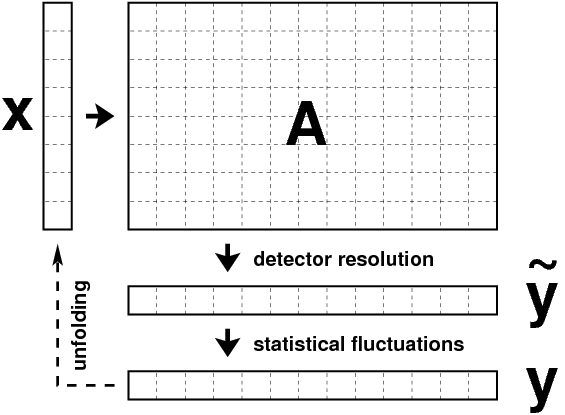
\includegraphics[width=0.4\textwidth]{06_DiffXsec/plots/d12-129f1.png}
  \caption{Schematic view of the problem of migration effects due to the finite precision of the detector and statistical 
  fluctuations. Plot taken from \cite{Schmitt:2012kp}.}
  \label{fig:scUnf}
\end{figure}

The most simple solution would be to take $y_{i}$ instead of $\tilde{y}_{i}$ in eq. \ref{eq:UnfoldProb} and invert
the $A_{ij}$ matrix to obtain $x_{j}$. But it turns out that the statistical fluctuations of $y_{i}$ are greatly 
amplified this way. To minify these fluctuations the \textit{regularisation} procedure is applied.

The process of restoring the true distribution $\tilde{x}_{j}$ from the known distribution $y_{i}$ which was influenced
by the detector effects and statistical fluctuations is called \textit{unfolding}. The TUnfold \cite{Schmitt:2012k} algorithm was used for the
unfolding in this work.

\subsection{Mathematical Background}

The TUnfold algorithm is using the least square minimization method and the Tikhonov regularization \cite{Tikhonov:1963}. One of the crucial 
constrains for a better performance of the method is that the number of degrees of freedom for the minimization ($n - m$) has to be positive,
or $n > m$. This means that the true unfolded distribution $\tilde{x}_j$ will have coarser binning than the measured one, $y_{i}$.

The unfolding algorithm of the TUnfold determines the stationary point of the Lagrangian:

\begin{align}
 \mathcal{L}(x, \lambda) = \mathcal{L}_{1} + \mathcal{L}_{2} + \mathcal{L}_{3}, \;\;\;\;\; \textrm{where}\\
 \mathcal{L}_{1} = (\mathbf{y} - \mathbf{A}\mathbf{x})^{T} \mathbf{V_{yy}}^{-1}(\mathbf{y} - \mathbf{A}\mathbf{x})
\end{align}


% \section{Cross Section Definition}
% \subsection{Total Production Cross Section}
% \subsection{Double Differential Production Cross Section}

% \chapter{Tracking Inefficiency due to Hadronic Interactions}\label{sect:hadr_interactions}
% \chaptermark{Tracking Inefficiency}
% 
% The charm and beauty measurement performed in this thesis relies on a proper detector simulation,
% since it is used to determine the acceptance as well as shapes of signal and background distributions.
% In particular, one of the most important requirements
% is a precise modelling of the tracking efficiency.
% There are several effects that lead to a tracking inefficiency,
% such as the detector efficiency, the pattern recognition efficiency 
% or the disappearance of tracks due to hadronic interactions with detector matter nuclei.
% The latter effect is a dominant contribution to the tracking inefficiency at ZEUS.
% A large uncertainty was associated to it.
% In order to reduce the resulting cross section systematic uncertainty, a dedicated study was performed within this thesis.
% It is described in detail in the following.
% 
% \section{Method}
% 
% The goal of the study is to check how well the probability of hadronic interactions\footnote{Shortly {\it interactions} in what follows.} is reproduced by the Monte Carlo (MC) simulation.
% This can be done by measuring a quantity which is sensitive to this effect and comparing it between data and MC.
% Any observed differences would point to an imperfect simulation of interactions.
% A correction can then be derived and applied to the MC.
% 
% Interactions in the transition region between the MVD and the CTD, i.e. in the outer wall of the MVD or the inner wall of the CTD,
% as well in the outer layers of the MVD, were considered.
% If no interaction occurs, a particle will leave hits in both MVD and CTD, hence a full-length track can be reconstructed.
% However, if a particle interacts hadronically with a nucleus in this detector region, it will disappear as a result of the corresponding reaction or will be significantly deflected from its original flight direction,
% and hence generally will not be detected by the CTD.
% However it still can be reconstructed in the MVD. We will denote such tracks, based only on MVD hits without
% a CTD counterpart, as MVDSA tracks (MVD Stand-Alone tracks).
% The relative fraction $R$ of such tracks with respect to all reconstructed tracks is directly sensitive to the probability of hadronic interaction in the MVD-CTD transition region.
% It is also related to the MVD and CTD acceptance which is assumed to be well simulated by the MC, thus it cancels out in the data-to-MC ratio if the assumption is correct.
% The other effect that can cause disappearance of tracks are in-flight particle decays. However, it is expected to be small compared to hadronic interactions.
% 
% Exclusive (diffractive) production of the $\rho(770)$-meson with a subsequent decay to two charged pions ($ep\to e'\rho\ p'$, $\rho\to\pi^+\pi^-$),
% was chosen as the type of events to be studied.
% In this process (see Fig.~\ref{fig:rho_diagram} for a Feynman diagram) the proton remains intact or dissociates into a low mass excited state and escapes the detector through the beam-pipe,
% hence only two charged pions, and possibly a scattered electron are detected.
% This is a very clean topology with practically no background (see Section~\ref{sect:selection}), which minimises possible systematic effects.
% 
% \begin{figure}[t]\label{fig:rho_diagram}\centering
%  \includegraphics[width=0.5\textwidth]{04_tracking_inefficiency_due_to_hadronic_interactions/plots/exclusive_rho.png}
% \caption{Feynman diagram of exclusive $\rho$ production at HERA}
% \end{figure}
% 
% If no interactions occur, there will be exactly two tracks (apart from the electron) coming from the primary vertex ({\it primary} tracks) which are well measured in the CTD ({\it long} tracks),
% as illustrated in the Figure~\ref{fig:classI}.
% However, if one of the pions interacts in the transition region, it can be reconstructed as an MVDSA track but not as a full-length track.
% Hence one expects one long primary track and one MVDSA track. Additionally, there might be other tracks due to particles that arise in the interaction, see Fig.~\ref{fig:classII}.
% However they cannot be attributed to the primary vertex, thus are easily distinguishable.
% For simplicity, we will call the first event type (with no interaction) as {\it class I}, while the second type (one of the pions interacts) will be denoted as {\it class II}.
% Cases when both pions interact are rare and were not considered.
% 
% \begin{figure}[t]
% 	\centering
% 	\subfigure[]{\label{fig:classI}
% 		\includegraphics[width=0.47\textwidth]{04_tracking_inefficiency_due_to_hadronic_interactions/plots/classI.png}
%     }
%     \subfigure[]{\label{fig:classII}
%     	\includegraphics[width=0.47\textwidth]{04_tracking_inefficiency_due_to_hadronic_interactions/plots/classII.png}
%     }
%   \caption{\label{fig:method_illustration} An illustration of the method. (a) Class I event topology. Both pions did not interact and hence are well measured
%     both in the MVD and the CTD (b) Class II event topology. One of the pions did not interact and is detected both in the MVD and the CTD. The other pion interacted in the MVD-CTD transition region and is reconstructed as an MVDSA track with no CTD counterpart (the original trajectory of the pion is shown as a dashed line).
%     Additional non-primary tracks emerging from the interaction point are also shown.} 
% \end{figure}
% 
% \section{Data and Monte Carlo Samples}\label{sect:data_mc_samples}
% 
% The full HERA II data sample, corresponding to an integrated luminosity of around \SI{354}{\per\pico\barn} was used for these studies.
% The DIS regime was chosen, since it provides a clean trigger signature thanks to the presence of the scattered electron.
% This is in contrast to the photoproduction mode where the electron is not detected, hence triggering of exclusive $\rho$ production events relies on the tracking information
% of the pions from the $\rho$ decay.
% 
% The \ZEUSVM~\cite{thesis:muchorowski:1996} Monte Carlo generator was used to generate $ep\to e\rho^0(\to\pi^+\pi^-) p$ events in DIS.
% Exclusive production and decay of the $\rho$-meson are characterised by event kinematic variables, the photon virtuality $Q^2$, the hadronic system mass $W$ and
% the four-momentum exchange at the proton vertex $t$ and by three helicity angles which are defined in the $\gamma^*p$-frame and in the $s$-channel helicity frame~\cite{wolf:1973, Chekanov:2007zr}.
% The $Q^2$ and $W$ distributions in \ZEUSVM are generated according to the Born cross-section for the process $\gamma^*p\to\rho^0 p$, where
% $\gamma^*$ denotes a virtual photon~\cite{thesis:kreisel:2004}.
% The minimum cut on $Q^2$ was \SI{1.5}{\GeV\squared}.
% The $t$ distribution is an exponential function with a slope set to $b=\SI{5}{\per\GeV\squared}$.
% Flat distributions of helicity angles are generated.
% \ZEUSVM was interfaced to \HERACLES~\cite{cpc:69:155} in order to take initial and final state QED radiation into account.
% 
% Table~\ref{tab:zeusvm_nevents} shows the number of events that were used for each data taking period.
% The MC events are processed in the same way as the data, i.e. the same reconstruction and selection procedures are applied. 
% 
% \begin{table}[t]
%   \centering
%   \begin{tabular}{|c|c|c|c|}
%     \hline
%     Period & Lepton Type & Integrated Luminosity, pb$^{-1}$ & Number of MC events \\ \hline
%     2003-2004 & e$^+$ & 30.61 & 740 289 \\ \hline
%     2005 & e$^-$ & 133.14 &  1 702 402\\ \hline
%     2006 & e$^-$ & 52.69 &  567 459\\ \hline
%     2006-2007 & e$^+$& 137.30 &  2 224 481 \\ \hline
%   \end{tabular}
%   \caption{Details on data and \ZEUSVM MC samples used in this chapter.}
%   \label{tab:zeusvm_nevents}
% \end{table}
% 
% \section{Selection}\label{sect:selection}
% 
% DIS events are characterised by a large scattering angle of the electron, which allows its detection in the main calorimeters.
% Hence, in order to select a DIS sample, a reconstructed electron candidate was required for each event.
% The SINISTRA algorithm (see Section~\ref{sect:sinistra}) was used to search and identify electrons.
% The following criteria, which are standard for ZEUS, were applied:
% \begin{itemize}
%  \item The presence of at least one SINISTRA electron candidate is required;
%  \item Electron probability $>\SI{90}{\percent}$ -- for each candidate, the algorithm assigns a certain probability for it to be caused by an electromagnetic cluster.
%                                         Only the most probable candidate is considered.
%                                         The cut on its probability ensures a good purity of electromagnetic showers identification;
%  \item Energy of the scattered electron $E_e'>\SI{10}{\GeV}$ -- suppresses fake electron candidates coming from e.g. pions decaying into photons and ensures good efficiency of the finder.
% \end{itemize}
% Further cleaning cuts were imposed:
% 
% \begin{itemize}
%  \item A reconstructed primary vertex with $|\zvtx|<\SI{30}{\cm}$ -- ensures that tracks emerging in collisions are in the CTD and MVD acceptance regions and  reduces non-$ep$ background;
%  \item $35<E-p_Z<\SI{70}{\GeV}$, where $E-p_Z=\sum_{i}\left(E - P_Z\right)_{i}$, the sum runs over all ZUFOs. For a fully reconstructed DIS event one expects $E-p_Z=2\,E_e=\SI{55}{\GeV}$~\footnote{
%  Due to the energy-momentum conservation, the quantity $E-p_Z$ is equal in the initial and final states.
%  Its calculation is straightforward in the former case:
%  the proton moves along the $Z$ axis, therefore it  does not contribute to $E-p_Z$ (since $E_p\approx (p_Z)_p$, neglecting the mass),
%  while the electron moves in the opposite direction and $E_e\approx-(p_Z)_e$.
%  Hence, in the initial state $(E-p_Z)_\text{in}\approx 2E_e$.
%  }.
%  The given cut reduces photoproduction and non-$ep$ background.
% \end{itemize}
% No other explicit cuts were applied to select DIS events. In particular, no specific trigger chains were required and no kinematic ($Q^2$, $W$, $t$) cuts were imposed, in order to maximise the statistics.
% Within the selected DIS sample, events with class I and class II topologies were searched for.
% 
% For class I events, two {\it long} tracks of opposite charge flagged as primary were required; definition of the long track is as follows:
% \begin{itemize}
%  \item A track starts in the first CTD superlayer or in the MVD;
%  \item A track reaches the third CTD superlayer;
%  \item $\delta<\SI{0.2}{\cm}$, where $\delta$ is the transverse impact parameter, that is the distance of closest approach between the track trajectory and the beam spot (see Section~\ref{sect:vertex}), in the plane transverse to the beam direction ($XY$-plane). This cut ensures that a track is consistent with coming from the primary vertex.
% \end{itemize}
% No other tracks apart from the electron were allowed in the event.
% 
% For the class II, only one primary long track is allowed, with the same criteria as for class I.
% Exactly one MVDSA track is required with the following properties:
% \begin{itemize}
%  \item Number of hits (sum of $r\phi$ and $rz$ hits) in the Barrel MVD (BMVD) $\ge$ 5 -- ensures that the track is measured in at least three MVD layers\footnote{As discussed in Section~\ref{sect:mvd}, each MVD layer provides one $r\phi$- and one $rz$-measurement (hit).};
%  \item Transverse impact parameter $\delta<\SI{0.2}{\cm}$.
% \end{itemize}
% This ensures a good measurement by the MVD and that the track is not a secondary one.
% Additionally, any number of tracks not flagged as primary is allowed for the class II, since they might come from the hadronic interaction.
% For both classes, the kinematic range for selected primary tracks (i.e. pion candidates) was:
% \begin{itemize}
%  \item $p_T>\SI{0.2}{\GeV}$ -- low momenta tracks might not reach the CTD due to bending in the magnetic field;
%  \item $0.44<\theta<\SI{2.7}{\radian}$ -- selects tracks in the acceptance region of the CTD. At higher or lower values of the polar angle, a track cannot pass three CTD layers.
% \end{itemize}
% In order to suppress the contamination from exclusive production of $\phi(1020)\to K^+K^-$ where kaons are misidentified as pions,
% events fulfilling $1.012<M(\phi)<\SI{1.028}{\GeV}$, where $M(\phi)$ is the mass of the two primary tracks (pion candidates) assuming kaon mass, are rejected.
% 
% Although the given criteria allow selection of a reasonably clean sample of exclusive $\rho$ events, there is still background, e.g.
% events when other particles in addition to the two pion candidates are produced in the $ep$-collision.
% For example, the exclusive production of the $\omega(782)$-meson with a subsequent decay $\omega\to\pi^+\pi^-\pi^0$ will also lead to only two reconstructed tracks in the event, since
% the neutral pion escapes detection by the tracking system. Hence these events can be accepted with the selection described above.
% Another example is non-exclusive production of the $\rho$-meson, when other particles in addition to the $\rho$ are produced.
% 
% In order to supress events with additional neutral particles, the so called {\it elasticity cut} is applied.
% It makes use of calorimeter information.
% In particular, if there are clusters of energy in the calorimeter which
% cannot be attributed to one of the two pions, such events are rejected.
% Matching of clusters to tracks is done by extrapolating a track to the calorimeter
% in order to obtain the impact position and the flight direction at the inner calorimeter surface.
% A straight track trajectory is assumed in CAL, since it is placed outside the solenoid and the magnetic field is much lower than in the tracking detectors (ranging typically from 0 to \SI{0.3}{\tesla}, but with local maxima of \SI{0.8}{\tesla})~\cite{Mainusch:1991sm}.
% Clusters closer to the track trajectory than \SI{30}{\cm} are considered as belonging to the track, i.e. {\it matched}. Clusters which are more distant are considered as not coming from the track or {\it unmatched}.
% Only clusters with energy deposit exceeding the calorimeter threshold of \SI{500}{\MeV} are considered.
% 
% For the class I, calorimeter clusters are allowed around both long tracks. If a cluster is found which is not matched to one of the two tracks, an event is rejected.
% For the class II, the situation is more complicated since hadronic interactions may lead to production of other tracks which would leave energy deposit in the calorimeter.
% In order to take this into account, calorimeter clusters which satisfy $\Delta R=\sqrt{(\eta^\text{trk}-\eta^\text{clus})^2+(\phi^\text{trk}-\phi^\text{clus})^2}<0.5$ are allowed, where $\eta^\text{trk}$~($\eta^\text{cluster}$) is the pseudorapidity
% of the MVDSA track (cluster) and $\phi^\text{trk}$~($\phi^\text{clus}$) is the azimuthal angle of the MVDSA track (cluster).
% Angles of the clusters are determined using the reconstructed primary vertex.
% For the long (non-interacted) track, clusters are matched in the same way as for class I.
% 
% After this selection, $\rho$-meson candidates are formed. For the class I, the $\rho$-candidate is reconstructed from two long primary tracks, while for the class II it is based on the long primary track and the MVDSA track.
% 
% \begin{figure}[!b]
% 
%   \centering
% 
%   \includegraphics[width=0.48\textwidth,height=0.35\textheight]{04_tracking_inefficiency_due_to_hadronic_interactions/plots/rho_mass_classI_data.png}
%   \includegraphics[width=0.48\textwidth,height=0.35\textheight]{04_tracking_inefficiency_due_to_hadronic_interactions/plots/rho_mass_classII_data.png}\\
%   \includegraphics[width=0.48\textwidth,height=0.35\textheight]{04_tracking_inefficiency_due_to_hadronic_interactions/plots/rho_mass_classI_MC.png}
%   \includegraphics[width=0.48\textwidth,height=0.35\textheight]{04_tracking_inefficiency_due_to_hadronic_interactions/plots/rho_mass_classII_MC.png}
% 
%   \caption{Mass distributions of $\rho(770)$ candidates for class I events (a), (c) and class II events (b), (d). Top row distributions are for data, bottom row plots are obtained from the MC.}
%   \label{fig:rho_masspeak}
% \end{figure}
% 
% Figure~\ref{fig:rho_masspeak}(a) shows the mass distribution for data for class I events after the event selection described above.
% A clear peak which can be attributed to exclusive production of the $\rho(770)$-meson is observed.
% The asymmetric form is due to the Breit-Wigner shape of the $\rho$-meson.
% Events in the range of $M(\pi^+\pi^-)\in[0.6,\ 1.1]\,\si{\GeV}$ were selected for further analysis.
% In this region, background from exclusive production of $\phi(1020)\to K^+K^-$ where kaons are misidentified as pions or $\omega(782)\to\pi^+\pi^-\pi^0$ is expected~\cite{Chekanov:2007zr} to be negligible.
% However, it contributes to the region of smaller $M(\pi^+\pi^-)$ which leads to an excess on the left of the peak. 
% The non-resonant background is expected to be at a level of \SI{1}{\percent}~\cite{Chekanov:2007zr}.
% 
% Figure~\ref{fig:rho_masspeak}(b) shows the  mass distribution for data for class II events.
% A clear peak can be observed with similar features as for class I, despite the fact that one of the pions is measured by the MVD only, hence the $\rho$ mass resolution is inferior compared to class~I.
% The statistics is worse than for class~I and this is a limiting factor of the method.
% 
% Figures~\ref{fig:rho_masspeak}(c)-(d) show the $\rho$ mass distributions for MC for class I and class II samples.
% Since the $\omega$ and $\phi$ background was not simulated, no excess is present at $M(\pi^+\pi^-)\lesssim\SI{0.6}{\GeV}$, as for the data.
% 
% \section{Monte Carlo Reweighting}\label{sect:rew}
% 
% The quality of the modelling of the $\rho$-meson decay products kinematics by the MC can influence results obtained with the method described in this chapter.
% For example, it was mentioned above that one of the assumptions is a correct description of the MVD acceptance for MVDSA tracks.
% Since it depends crucially on the track kinematics, the latter has to be well described by the MC.
% 
% However it is known that the \ZEUSVM MC does not provide a good description of the process kinematics.
% As discussed in Section~\ref{sect:data_mc_samples}, flat distributions for helicity angles are generated, which do not correspond to the measured ones~\cite{Chekanov:2007zr}.
% Event kinematic variables ($Q^2$, $W$, $t$) are not well described as well~\cite{Chekanov:2007zr}.
% Both effects spoil the description of the daughter products kinematics.
% 
% In order to reach a better agreement between data and MC, it is necessary to reweight the MC.
% The reweighting parametrisations are determined from the high statistics class~I sample and are then applied both for class~I and class~II MC samples.
% One possibility is to reweight the helicity angles using the spin-density matrix elements as a function of $Q^2$~\cite{Chekanov:2007zr}.
% However for our purpose it is sufficient to describe only the daughter products kinematics of the $\rho$-meson,
% since the method described in this chapter is based on the detection of these particles.
% Hence, no attempt is made to perfectly describe the event kinematics and all of the helicity angles but
% rather to describe the $\rho$-meson kinematics and decay angles in its rest frame.
% This is sufficient to provide a good description of the daughter pion kinematics.
% In contrast, the helicity angles approach requires in general also a good understanding of the $Q^2, W$ and $t$ variables since the angles are defined in the $\gamma^*p$-frame.
% 
% \begin{figure}[p]
%   \centering
%     \subfigure[]{\label{fig:cos_theta_star_unrew}
%       \includegraphics[width=0.47\textwidth,height=0.35\textheight]{04_tracking_inefficiency_due_to_hadronic_interactions/plots/cos_theta_star_classI.png}
%     }
%     \subfigure[]{\label{fig:cos_theta_star_rew}
%       \includegraphics[width=0.47\textwidth,height=0.35\textheight]{04_tracking_inefficiency_due_to_hadronic_interactions/plots/cos_theta_star_classI_rew.png}
%     }
%     \caption{The $\cth$~distribution for class~I before (a) and after (b) reweighting. The points show the data, the histogram represents the MC. MC was normalised to data area.}
%     \label{fig:cos_theta_star} 
%     \subfigure[]{
%       \includegraphics[width=0.47\textwidth,height=0.35\textheight]{04_tracking_inefficiency_due_to_hadronic_interactions/plots/pi_plus_pt_classI.png}
%     }
%     \subfigure[]{
%       \includegraphics[width=0.47\textwidth,height=0.35\textheight]{04_tracking_inefficiency_due_to_hadronic_interactions/plots/pi_plus_pt_classI_rew.png}
%     }
%     \caption{\label{fig:pt_plus}The distributions of the transverse momentum of the positive pion, $p_T(\pi^+)$, for class I events before the $\cth$~reweighting (a)  and after it (b).
%              The points show the data, the histogram represents the MC. MC was normalised to data area.} 
% \end{figure}
% 
% We define $\theta^*$ as the angle between the positive track and the $\rho$ direction, in the $\rho$ rest frame.
% It is obtained as follows: the laboratory frame is rotated such that its $z$ axis coincides with the $\rho$ direction, then a boost
% along the $z$ direction to the $\rho$ rest frame is performed.
% %$\theta^*$ is the polar angle of the positive pion in this frame.
% Figure~\ref{fig:cos_theta_star} shows the $\cth$ distribution for data and MC, for class~I events. The MC was normalised to data area.
% One is forced to conclude that the data and the MC have very different shapes, hence the MC is reweighted.
% The following reweighting function was obtained from this distribution:
% $$\zeta(\cth) = 0.284 + 0.00138\cth + 2.67(\cth)^2$$
% The $\cth$  distribution after application of this reweighting is shown in Fig.~\ref{fig:cos_theta_star_rew}.
% A good agreement is observed.
% The observable $\theta^*$ has direct influence on the kinematics of the daughter products in the laboratory frame.
% Fig.~\ref{fig:pt_plus} shows the transverse momentum distribution of the positive pion for class I before and after $\cth$-reweighting.
% The agreement becomes much better after reweighting.
% 
% The azimuthal angle of the scattered electron as well as that of the $\rho$ meson are not well described by the MC.
% One of the possible reasons is that in the MC, no trigger requirements were imposed, while data must be always accepted by certain trigger slots, mostly by the inclusive DIS triggers.
% The fact that the efficiency of these triggers might depend on the azimuthal angle, especially at low electron scattering angles (due to the electron box cut), may lead to such a discrepancy.
% In order to correct for this, a reweighting in the azimuthal angle $\phi$ of the $\rho$-meson is performed with the following parametrisation:
% $$\xi(\phi) = 1.28 - 0.33\,\phi + 0.080\,\phi^2 + 0.0123\,\phi^3 - 0.050\,\phi^4 - 0.0011\,\phi^5 + 0.0039\,\phi^6$$
% The high order of the polynomial is necessary to account for the shape of the data-to-MC ratio.
% After this reweighting, the azimuthal distribution of the scattered electron, the $\rho$~meson and its decay products is significantly improved (see Section~\ref{sect:trk.cplots}).
% 
% In summary, each MC event gets a weight $w=\zeta(\cth)\,\xi(\phi)$ with $\theta^*$ and $\phi$ defined on the true MC level.
% 
% \section{Control Distributions}\label{sect:trk.cplots}
% 
% As discussed in the previous section, it is necessary to check whether the MC describes the data reasonably,
% and to understand, whether remaining differences (if any) influence the results.
% In this section, various distributions are compared between data and MC. For all plots, MC was normalised to the data.
% 
% Figure~\ref{fig:rho_pi_classI} shows the distributions of the transverse momentum~$p_T$, the polar angle~$\theta$ and the azimuthal angle~$\phi$ of the $\rho$ meson and of its positive decay product ($\pi^+$) for class~I events.
% All quantities are calculated in the laboratory frame. The distributions for $\pi^-$  are very similar to those of $\pi^+$.
% A reasonable agreement between the data and the MC simulation is observed.
% However some discrepancies are present for $p_T(\rho)$, Fig.~\ref{fig:rho_pi_classI}(a), for $\theta(\rho)$, Fig.~\ref{fig:rho_pi_classI}(b) and for $p_T(\pi^+)$, Fig.~\ref{fig:rho_pi_classI}(d).
% They can arise due to the imperfect simulation of the $\rho$ meson kinematics and as well as of the helicity angles (see Section~\ref{sect:rew}).
% The deficit of the MC at low $p_T(\rho)$, Fig.~\ref{fig:rho_pi_classI}(a), can be also associated to additional background in data.
% It was checked that results obtained in this chapter do not change significantly if these differences are removed by reweighting of a corresponding variable or by removing the 
% region below $p_T(\rho)=\SI{1.3}{\GeV}$, where the excess of the data is present (see Section~\ref{sect:trk_eff_results}).
% 
% Figure~\ref{fig:rho_ZTT_classII} shows the kinematic variables ($p_T$, $\theta$ and $\phi$) of the $\rho$ meson and of the long primary track for the class~II sample.
% Similarly to class~I, the MC undershoots the data at low values of the $\rho$ transverse momentum.
% No other significant discrepancies are observed within statistical uncertainties.
% Figures~\ref{fig:MSA_classII}(a)-(c) show the kinematic variables of the MVDSA track in class II events.
% Somewhat different shapes are observed compared to the long tracks distributions, which can be attributed to the MVD acceptance.
% The MC describes the data well.
% Figures~\ref{fig:MSA_classII}(d)-(e) show the number of hits in the Barrel MVD (BMVD) for MVDSA tracks in class~II events.
% Excellent agreement of the data and the MC suggests good understanding of the MVD hit efficiency which was assumed so far.
% Figure~\ref{fig:MSA_imppar_classII} shows the distribution of the transverse and $z$-impact parameters for the MVDSA track for class~II events.
% Similar shapes are observed for data and MC, hence the selected MVDSA tracks are consistent with real primary tracks and are not due to background.
% There is also some discrepancy which could arise due to the fact that not the latest alignment corrections were applied for the MVDSA track reconstruction algorithm~\cite{gerd}.
% 
% Figure~\ref{fig:long_tracks_classII}(a) shows the multiplicity distribution for the long tracks (those starting at or before the first CTD superlayer and passing at least three superlayers) for class II,
% including the non-interacted pion.
% The MC reasonably reproduces the distribution, in particular the fact that there are often several non-primary tracks.
% Some discrepancies are visible for cases with one and two long tracks.
% This can happen if the probability of certain hadronic reactions is not well simulated. This is exactly an effect searched for and does not pose a problem.
% The transverse impact parameter distribution for the long tracks (excluding the non-interacted pion) is shown in Fig.~\ref{fig:long_tracks_classII}(b).
% It is very broad as expected for secondary tracks. The description by the MC is reasonable, indicating that there is no significant pollution from e.g. primary tracks to this sample.
% 
% In summary, the MC describes reasonably the properties of the $\rho$ meson and of its decay products for both class~I and class~II samples.
% The remaining differences in track kinematics do not affect the results of this chapter significantly, which was verified by several checks (see Section~\ref{sect:trk_eff_results}).
% 
% \begin{figure}[p]
%   \centering
%     \begin{overpic}[width=0.494\textwidth]{04_tracking_inefficiency_due_to_hadronic_interactions/plots/control_plots/classI/rho_pt_classI.png}
%     \put(50,67){(a)}
%     \end{overpic}
%     \begin{overpic}[width=0.494\textwidth]{04_tracking_inefficiency_due_to_hadronic_interactions/plots/control_plots/classI/rho_theta_classI.png}
%     \put(50,67){(b)}
%     \end{overpic}\\
%     \begin{overpic}[width=0.494\textwidth]{04_tracking_inefficiency_due_to_hadronic_interactions/plots/control_plots/classI/rho_phi_classI.png}
%     \put(50,67){(c)}
%     \end{overpic}
%     \begin{overpic}[width=0.494\textwidth]{04_tracking_inefficiency_due_to_hadronic_interactions/plots/control_plots/classI/pi_plus_pt_classI.png}
%     \put(50,67){(d)}
%     \end{overpic}\\
%     \begin{overpic}[width=0.494\textwidth]{04_tracking_inefficiency_due_to_hadronic_interactions/plots/control_plots/classI/pi_plus_theta_classI.png}
%     \put(50,67){(e)}
%     \end{overpic}
%     \begin{overpic}[width=0.494\textwidth]{04_tracking_inefficiency_due_to_hadronic_interactions/plots/control_plots/classI/pi_plus_phi_classI.png}
%     \put(40,67){(f)}
%     \end{overpic}
%     \caption{Control plots for the class~I sample: the transverse momentum (a), the polar angle (b) and the azimuthal angle (c) of the $\rho$ candidate;
%               the transverse momentum (d), the polar angle (e) and the azimuthal angle (f) of the positive pion. The points show the data, the histogram represents the MC.}
%     \label{fig:rho_pi_classI} 
% \end{figure}
% 
% \begin{figure}[p]
%   \centering
%     \begin{overpic}[width=0.493\textwidth]{04_tracking_inefficiency_due_to_hadronic_interactions/plots/control_plots/classII/rho_pt_classII.png}
%     \put(20,67){(a)}
%     \end{overpic}
%     \begin{overpic}[width=0.493\textwidth]{04_tracking_inefficiency_due_to_hadronic_interactions/plots/control_plots/classII/rho_theta_classII.png}
%     \put(20,67){(b)}
%     \end{overpic}\\
%     \begin{overpic}[width=0.493\textwidth]{04_tracking_inefficiency_due_to_hadronic_interactions/plots/control_plots/classII/rho_phi_classII.png}
%     \put(20,67){(c)}
%     \end{overpic}
%     \begin{overpic}[width=0.493\textwidth]{04_tracking_inefficiency_due_to_hadronic_interactions/plots/control_plots/classII/pi_ZTT_pt_classII.png}
%     \put(20,67){(d)}
%     \end{overpic}\\
%     \begin{overpic}[width=0.493\textwidth]{04_tracking_inefficiency_due_to_hadronic_interactions/plots/control_plots/classII/pi_ZTT_theta_classII.png}
%     \put(20,67){(e)}
%     \end{overpic}
%     \begin{overpic}[width=0.493\textwidth]{04_tracking_inefficiency_due_to_hadronic_interactions/plots/control_plots/classII/pi_ZTT_phi_classII.png}
%     \put(60,67){(f)}
%     \end{overpic}
%     \caption{Control plots for the class~II sample: the transverse momentum (a), the polar angle (b) and the azimuthal angle (c) of the $\rho$ candidate;
%               the transverse momentum (d), the polar angle (e) and the azimuthal angle (f) of the pion which did not interact (long track).
%               The points show the data, the histogram represents the MC.}
%     \label{fig:rho_ZTT_classII} 
% \end{figure}
% 
% \begin{figure}[p]
%   \centering
%     \begin{overpic}[width=0.494\textwidth]{04_tracking_inefficiency_due_to_hadronic_interactions/plots/control_plots/classII/pi_MSA_pt_classII.png}
%     \put(60,65){(a)}
%     \end{overpic}
%     \begin{overpic}[width=0.494\textwidth]{04_tracking_inefficiency_due_to_hadronic_interactions/plots/control_plots/classII/pi_MSA_theta_classII.png}
%     \put(55,65){(b)}
%     \end{overpic}\\
%     \begin{overpic}[width=0.494\textwidth]{04_tracking_inefficiency_due_to_hadronic_interactions/plots/control_plots/classII/pi_MSA_phi_classII.png}
%     \put(60,65){(c)}
%     \end{overpic}
%     \begin{overpic}[width=0.494\textwidth]{04_tracking_inefficiency_due_to_hadronic_interactions/plots/control_plots/classII/pi_MSA_Trkmsa_nbr_classII.png}
%     \put(60,65){(d)}
%     \end{overpic}\\
%     \begin{overpic}[width=0.494\textwidth]{04_tracking_inefficiency_due_to_hadronic_interactions/plots/control_plots/classII/pi_MSA_Trkmsa_nbz_classII.png}
%     \put(60,65){(e)}
%     \end{overpic}
%     \caption{Control plots for the MVDSA track, class~II. Shown are the transverse momentum (a), the polar angle (b), the azimuthal angle (c), the number of $r$-hits in the Barrel MVD (BMVD) (d) and the number of $z$-hits in BMVD (e). The points show the data, the histogram represents the MC.}
%     \label{fig:MSA_classII} 
% \end{figure}
% 
% \begin{figure}[t]
%   \centering
%     \begin{overpic}[width=0.495\textwidth]{04_tracking_inefficiency_due_to_hadronic_interactions/plots/control_plots/classII/pi_MSA_Trkmsa_imppar_classII.png}
%     \put(80,67){(a)}
%     \end{overpic}
%     \begin{overpic}[width=0.495\textwidth]{04_tracking_inefficiency_due_to_hadronic_interactions/plots/control_plots/classII/pi_MSA_z_imppar_classII.png}
%     \put(80,67){(b)}
%     \end{overpic}
%     \caption{Control plots for the MVDSA track, class~II. Shown are the transverse impact parameter with respect to the beam spot (a) and the $z$-impact parameter (b).
%             The points show the data, the histogram represents the MC.}
%     \label{fig:MSA_imppar_classII} 
% \end{figure}
% 
% \begin{figure}[!h]
%   \centering
%     \begin{overpic}[width=0.495\textwidth]{04_tracking_inefficiency_due_to_hadronic_interactions/plots/control_plots/classII/long_ZTT_tracks_classII.png}
%     \put(80,67){(a)}
%     \end{overpic}
%     \begin{overpic}[width=0.495\textwidth]{04_tracking_inefficiency_due_to_hadronic_interactions/plots/control_plots/classII/long_tracks_imppar_classII.png}
%     \put(80,67){(b)}
%     \end{overpic}\\
%     \caption{The number of long tracks including the non-interacted pion (a) and the transverse impact parameter of all secondary long tracks, excluding the non-interacted pion (b).
%             Both distributions are for the class~II sample.
%             The points show the data, the histogram represents the MC.}
%   \label{fig:long_tracks_classII} 
% \end{figure}
% 
% \clearpage
% 
% \section{Results}\label{sect:trk_eff_results}
% 
% This section presents results of the hadronic interactions investigation. Two types of observables are constructed and studied: the {\it single ratio} and the {\it double ratio}.
% 
% The {\it single ratio}, $R$, is defined in the following way:
% $$R(x_i)=\frac{N_\text{MVDSA}(x_i)}{N_\text{long, primary}(x_i)+N_\text{MVDSA}(x_i)}.$$
% Here $N_\text{MVDSA}(x_i)$ is the number of MVDSA tracks within the class II which are in the bin $i$ of some track or event variable $x$, e.g. track $p_T$;
% $N_\text{long, primary}(x_i)$ is the total number of long primary tracks in the bin $i$ both from class I and class II.
% If the variable $x$ is not required to be in the bin $i$ (or it is an event variable), there will be  two long primary tracks and no MVDSA tracks in class~I events ($N_\text{long, primary}=2$, $N_\text{MVDSA}=0$)
% while for class~II events there will be one long primary and one MVDSA track ($N_\text{long, primary}=1$, $N_\text{MVDSA}=1$).
% 
% The single ratio $R$ determined in this way is proportional to the probability for a track to interact hadronically in the MVD-CTD
% transition region and to the MVD acceptance for MVDSA tracks.
% Assuming that the latter is well modelled by the Monte Carlo, it is useful to construct the {\it double ratio}:
% $$\epsilon(x)=\frac{R_\text{DATA}(x)}{R_\text{MC}(x)},$$
% where $R_\text{DATA}(x)$ and $R_\text{MC}(x)$ are the single ratio obtained for data and Monte Carlo respectively.
% This quantity is a direct measure of how well the hadronic interaction probability is simulated by the MC and is the main observable in this method.
% 
% Figures~\ref{fig:r}(a)-(f) show results for the single ratio $R$ for data and MC as a function of the
% track azimuthal angle $\phi$, polar angle $\theta$ and transverse momentum $p_T$.
% Generally, a similar behaviour is observed in data and MC. In the azimuthal angle distribution,
% there are dips around $\phi=\SI{0}{\radian}$ and $\phi=\pm\SI{\pi}{\radian}$ which are regions of reduced MVD acceptance.
% The $\theta$ distributions are smooth and show a slow rise towards the backward direction.
% Finally, the $p_T$ distribution shows a steep rise towards low momenta.
% 
% Figure~\ref{fig:epsilon} shows the double ratio $\epsilon$ for the same kinematic variables.
% It follows that on average the Monte Carlo underestimates the interaction probability.
% The effect is consistent with a constant as a function of track angles $\phi$ and $\theta$.
% It has a more pronounced structure as a function of $p_T$.
% A fit with a constant is performed for the whole range in $\phi$ and $\theta$.
% The fit yields $\epsilon_\phi=1.29\pm0.04$ and $\epsilon_\theta=1.33\pm0.04$ for $\phi$ and $\theta$ respectively. The values are consistent with each other.
% Based on the observations from the $p_T$ distribution, the following model is proposed: the variable $\epsilon$ is consistent with constants for $p_T<\SI{1.5}{\GeV}$ and for $p_T>\SI{1.5}{\GeV}$,
% however the constants are different in these momenta regions.
% Hence, the $p_T$ distribution is fitted with a constant separately for $p_T<\SI{1.5}{\GeV}$ and for $p_T>\SI{1.5}{\GeV}$; a good quality of the fit suggests that this model is consistent with data.
% The fit yields $\epsilon_{p_T<\SI{1.5}{\GeV}}=1.36\pm0.05$ and $\epsilon_{p_T>\SI{1.5}{\GeV}}=0.96\pm0.09$ respectively.
% The latter number is consistent with unity with a \SI{10}{\percent} uncertainty, hence at this level of precision no deviation of MC from data is observed.
% However, at transverse momenta below \SI{1.5}{\GeV}, the MC underestimates the probability of hadronic interactions.
% 
% Several checks were performed in order to assess the stability of the result.
% Distributions of $\pT(\rho)$ and of $\theta(\rho)$ were reweighted in the MC, such that they reproduced the data, in order to take into account improper description of the $\rho$ kinematics;
% a cut of $\pT(\rho)>\SI{1.3}{\GeV}$ was applied in order to remove the region where there is a discrepancy between data and MC, Fig.~\ref{fig:rho_pi_classI}(a);
% the calorimeter noise threshold for the elasticity cut was lowered to \SI{300}{\MeV};
% the maximum allowed distance between the track and the island was lowered to \SI{20}{\cm};
% the cone radius around the MVDSA track for the elasticity cut, $\Delta R$, was varied by 0.3 (i.e. lowered to 0.2 and increased to 0.8);
% a cut of $Q^2_\text{da}>\SI{5}{\GeV\squared}$ was applied;
% the lower cut on the $\rho$ mass was increased to \SI{0.65}{\GeV}.
% The biggest change of the result comes from the variation of the calorimeter noise threshold ($\epsilon_{p_T<\SI{1.5}{\GeV}}=1.25$ and $\epsilon_{p_T>\SI{1.5}{\GeV}}=0.8$)
% and of the cone radius for the elasticity cut ($\epsilon_{p_T<\SI{1.5}{\GeV}}=1.24$ and $\epsilon_{p_T>\SI{1.5}{\GeV}}=0.86$ for $\Delta R=0.2$ and $\epsilon_{p_T<\SI{1.5}{\GeV}}=1.51$ and $\epsilon_{p_T>\SI{1.5}{\GeV}}=1.06$ for $\Delta R=0.8$).
% Other variations do not affect the result significantly. Based on this, the uncertainty on both $\epsilon_{p_T<\SI{1.5}{\GeV}}$ and $\epsilon_{p_T>\SI{1.5}{\GeV}}$ is estimated to be around $\pm0.2$.
% 
% \begin{figure}[p]
%   \centering
%     \begin{overpic}[width=0.9\textwidth]{04_tracking_inefficiency_due_to_hadronic_interactions/plots/results/phi_R_v136.png}
%     \put(30,35){(a)}
%     \put(90,35){(b)}
%     \end{overpic}\\
%     \begin{overpic}[width=0.9\textwidth]{04_tracking_inefficiency_due_to_hadronic_interactions/plots/results/theta_R_v136.png}
%     \put(30,35){(c)}
%     \put(90,35){(d)}
%     \end{overpic}\\
%     \begin{overpic}[width=0.9\textwidth]{04_tracking_inefficiency_due_to_hadronic_interactions/plots/results/pt_R_v136.png}
%     \put(30,35){(e)}
%     \put(90,35){(f)}
%     \end{overpic}
%    \caption{Single ratio $R$ (see text for the definition) for data (left column) and MC (right column) as a function of the azimuthal angle $\phi$ (a)-(b), the polar angle $\theta$ (c)-(d) and the transverse momentum $p_T$ (e)-(f) of the track.}
%   \label{fig:r}
% \end{figure}
% 
% \begin{figure}[p]\centering
% 	\subfigure[]{
%       \includegraphics[width=0.47\textwidth]{04_tracking_inefficiency_due_to_hadronic_interactions/plots/results/phi_epsilon_v136.png}
%     }
% 	\subfigure[]{
%       \includegraphics[width=0.47\textwidth]{04_tracking_inefficiency_due_to_hadronic_interactions/plots/results/theta_epsilon_v136.png}
%     }
% 	\subfigure[]{\label{fig:epsilon_pt}
%       \includegraphics[width=0.5\textwidth]{04_tracking_inefficiency_due_to_hadronic_interactions/plots/results/pt_epsilon_v136.png}
%     }
%   \caption{Double ratio $\epsilon$ (see text for the definition) as a function of the polar angle $\phi$ (a), the azimuthal angle $\theta$ (b) and the transverse momentum $p_T$ (c) of the track.}
%   \label{fig:epsilon}
% \end{figure}
% 
% \clearpage
% 
% \section{Summary}
% 
% In this chapter, the quality of the hadronic interactions modelling by the MC was studied.
% It was found that on average the MC underestimates the probability of interactions.
% The effect depends on transverse momentum $p_T$ of the track. At low momenta of $p_T<\SI{1.5}{\GeV}$, it is underestimated by a factor of $\sim1.4$, while for $p_T>\SI{1.5}{\GeV}$ a good description is observed.
% 
% One of the reasons for underestimation of hadronic interaction probability might be an imperfect simulation of cross-sections of certain reactions.
% An example could be the production of the $\Delta(1232)$ resonance:
% $$\pi+p\to\Delta(1232)$$
% The highest cross-section for this reaction is at the centre-of-mass energy of the pion-proton system close to the mass of the $\Delta$-baryon,
% i.e. for pion momenta below \SI{1}{\GeV} if the proton is at rest. If MC underestimates the cross-section, this will lead to an underestimation of the interaction probability for pion momenta below \SI{1}{\GeV}.
% The other reason could be that the cross-section parametrisation used in \geant~\cite{tech:CERN:DDEE84-1,Brun:1994aa} is valid only at incident particle momentum of more than \SI{2}{\GeV}.
% 
% In order to take the observed difference into account, a correction has to be applied to the hadronic interaction probability in the MC. According to the results, a $p_T$-dependent correction must be used.
% No correction is applied for momenta above \SI{1.5}{\GeV}. A correction of $1.36$ is applied for $p_T<\SI{1.5}{\GeV}$.
% An uncertainty of $\pm0.2$ is assigned to the correction in both momentum regions, based on the effects of the procedure variations.